\documentclass[]{article}
\usepackage{lmodern}
\usepackage{amssymb,amsmath}
\usepackage{ifxetex,ifluatex}
\usepackage{fixltx2e} % provides \textsubscript
\ifnum 0\ifxetex 1\fi\ifluatex 1\fi=0 % if pdftex
  \usepackage[T1]{fontenc}
  \usepackage[utf8]{inputenc}
\else % if luatex or xelatex
  \ifxetex
    \usepackage{mathspec}
  \else
    \usepackage{fontspec}
  \fi
  \defaultfontfeatures{Ligatures=TeX,Scale=MatchLowercase}
\fi
% use upquote if available, for straight quotes in verbatim environments
\IfFileExists{upquote.sty}{\usepackage{upquote}}{}
% use microtype if available
\IfFileExists{microtype.sty}{%
\usepackage{microtype}
\UseMicrotypeSet[protrusion]{basicmath} % disable protrusion for tt fonts
}{}
\usepackage[margin=1in]{geometry}
\usepackage{hyperref}
\hypersetup{unicode=true,
            pdftitle={HW3},
            pdfauthor={Zihao\_Wang},
            pdfborder={0 0 0},
            breaklinks=true}
\urlstyle{same}  % don't use monospace font for urls
\usepackage{color}
\usepackage{fancyvrb}
\newcommand{\VerbBar}{|}
\newcommand{\VERB}{\Verb[commandchars=\\\{\}]}
\DefineVerbatimEnvironment{Highlighting}{Verbatim}{commandchars=\\\{\}}
% Add ',fontsize=\small' for more characters per line
\usepackage{framed}
\definecolor{shadecolor}{RGB}{248,248,248}
\newenvironment{Shaded}{\begin{snugshade}}{\end{snugshade}}
\newcommand{\KeywordTok}[1]{\textcolor[rgb]{0.13,0.29,0.53}{\textbf{#1}}}
\newcommand{\DataTypeTok}[1]{\textcolor[rgb]{0.13,0.29,0.53}{#1}}
\newcommand{\DecValTok}[1]{\textcolor[rgb]{0.00,0.00,0.81}{#1}}
\newcommand{\BaseNTok}[1]{\textcolor[rgb]{0.00,0.00,0.81}{#1}}
\newcommand{\FloatTok}[1]{\textcolor[rgb]{0.00,0.00,0.81}{#1}}
\newcommand{\ConstantTok}[1]{\textcolor[rgb]{0.00,0.00,0.00}{#1}}
\newcommand{\CharTok}[1]{\textcolor[rgb]{0.31,0.60,0.02}{#1}}
\newcommand{\SpecialCharTok}[1]{\textcolor[rgb]{0.00,0.00,0.00}{#1}}
\newcommand{\StringTok}[1]{\textcolor[rgb]{0.31,0.60,0.02}{#1}}
\newcommand{\VerbatimStringTok}[1]{\textcolor[rgb]{0.31,0.60,0.02}{#1}}
\newcommand{\SpecialStringTok}[1]{\textcolor[rgb]{0.31,0.60,0.02}{#1}}
\newcommand{\ImportTok}[1]{#1}
\newcommand{\CommentTok}[1]{\textcolor[rgb]{0.56,0.35,0.01}{\textit{#1}}}
\newcommand{\DocumentationTok}[1]{\textcolor[rgb]{0.56,0.35,0.01}{\textbf{\textit{#1}}}}
\newcommand{\AnnotationTok}[1]{\textcolor[rgb]{0.56,0.35,0.01}{\textbf{\textit{#1}}}}
\newcommand{\CommentVarTok}[1]{\textcolor[rgb]{0.56,0.35,0.01}{\textbf{\textit{#1}}}}
\newcommand{\OtherTok}[1]{\textcolor[rgb]{0.56,0.35,0.01}{#1}}
\newcommand{\FunctionTok}[1]{\textcolor[rgb]{0.00,0.00,0.00}{#1}}
\newcommand{\VariableTok}[1]{\textcolor[rgb]{0.00,0.00,0.00}{#1}}
\newcommand{\ControlFlowTok}[1]{\textcolor[rgb]{0.13,0.29,0.53}{\textbf{#1}}}
\newcommand{\OperatorTok}[1]{\textcolor[rgb]{0.81,0.36,0.00}{\textbf{#1}}}
\newcommand{\BuiltInTok}[1]{#1}
\newcommand{\ExtensionTok}[1]{#1}
\newcommand{\PreprocessorTok}[1]{\textcolor[rgb]{0.56,0.35,0.01}{\textit{#1}}}
\newcommand{\AttributeTok}[1]{\textcolor[rgb]{0.77,0.63,0.00}{#1}}
\newcommand{\RegionMarkerTok}[1]{#1}
\newcommand{\InformationTok}[1]{\textcolor[rgb]{0.56,0.35,0.01}{\textbf{\textit{#1}}}}
\newcommand{\WarningTok}[1]{\textcolor[rgb]{0.56,0.35,0.01}{\textbf{\textit{#1}}}}
\newcommand{\AlertTok}[1]{\textcolor[rgb]{0.94,0.16,0.16}{#1}}
\newcommand{\ErrorTok}[1]{\textcolor[rgb]{0.64,0.00,0.00}{\textbf{#1}}}
\newcommand{\NormalTok}[1]{#1}
\usepackage{graphicx,grffile}
\makeatletter
\def\maxwidth{\ifdim\Gin@nat@width>\linewidth\linewidth\else\Gin@nat@width\fi}
\def\maxheight{\ifdim\Gin@nat@height>\textheight\textheight\else\Gin@nat@height\fi}
\makeatother
% Scale images if necessary, so that they will not overflow the page
% margins by default, and it is still possible to overwrite the defaults
% using explicit options in \includegraphics[width, height, ...]{}
\setkeys{Gin}{width=\maxwidth,height=\maxheight,keepaspectratio}
\IfFileExists{parskip.sty}{%
\usepackage{parskip}
}{% else
\setlength{\parindent}{0pt}
\setlength{\parskip}{6pt plus 2pt minus 1pt}
}
\setlength{\emergencystretch}{3em}  % prevent overfull lines
\providecommand{\tightlist}{%
  \setlength{\itemsep}{0pt}\setlength{\parskip}{0pt}}
\setcounter{secnumdepth}{0}
% Redefines (sub)paragraphs to behave more like sections
\ifx\paragraph\undefined\else
\let\oldparagraph\paragraph
\renewcommand{\paragraph}[1]{\oldparagraph{#1}\mbox{}}
\fi
\ifx\subparagraph\undefined\else
\let\oldsubparagraph\subparagraph
\renewcommand{\subparagraph}[1]{\oldsubparagraph{#1}\mbox{}}
\fi

%%% Use protect on footnotes to avoid problems with footnotes in titles
\let\rmarkdownfootnote\footnote%
\def\footnote{\protect\rmarkdownfootnote}

%%% Change title format to be more compact
\usepackage{titling}

% Create subtitle command for use in maketitle
\newcommand{\subtitle}[1]{
  \posttitle{
    \begin{center}\large#1\end{center}
    }
}

\setlength{\droptitle}{-2em}
  \title{HW3}
  \pretitle{\vspace{\droptitle}\centering\huge}
  \posttitle{\par}
  \author{Zihao\_Wang}
  \preauthor{\centering\large\emph}
  \postauthor{\par}
  \predate{\centering\large\emph}
  \postdate{\par}
  \date{11/13/2018}


\begin{document}
\maketitle

\begin{Shaded}
\begin{Highlighting}[]
\KeywordTok{rm}\NormalTok{(}\DataTypeTok{list=}\KeywordTok{ls}\NormalTok{())}
\KeywordTok{set.seed}\NormalTok{(}\DecValTok{12345}\NormalTok{)}
\KeywordTok{options}\NormalTok{(}\DataTypeTok{warn =} \OperatorTok{-}\DecValTok{1}\NormalTok{)}
\NormalTok{knitr}\OperatorTok{::}\NormalTok{opts_knit}\OperatorTok{$}\KeywordTok{set}\NormalTok{(}\DataTypeTok{root.dir =} \StringTok{'~/Desktop/stat374-fall-2018/analysis/'}\NormalTok{)}
\KeywordTok{suppressMessages}\NormalTok{(}\KeywordTok{library}\NormalTok{(kedd))}
\KeywordTok{suppressMessages}\NormalTok{(}\KeywordTok{library}\NormalTok{(fields))}
\KeywordTok{suppressMessages}\NormalTok{(}\KeywordTok{library}\NormalTok{(}\StringTok{"tidyverse"}\NormalTok{))}
\end{Highlighting}
\end{Shaded}

\section{1 Chicago Crime}\label{chicago-crime}

\begin{Shaded}
\begin{Highlighting}[]
\CommentTok{# crime = read.csv("../data/hw3/Crimes_-_Map.csv")}
\CommentTok{# crime_loc = crime[,c("LATITUDE","LONGITUDE")]}
\CommentTok{# saveRDS(crime_loc, "../data/hw3/crime_loc.rds")}
\NormalTok{crime_loc =}\StringTok{ }\KeywordTok{readRDS}\NormalTok{(}\StringTok{"../data/hw3/crime_loc.rds"}\NormalTok{)}
\NormalTok{## remove samples with NA}
\NormalTok{crime_loc =}\StringTok{ }\KeywordTok{na.omit}\NormalTok{(crime_loc)}
\end{Highlighting}
\end{Shaded}

\begin{Shaded}
\begin{Highlighting}[]
\CommentTok{# set.seed(12345)}
\CommentTok{# ## take a small sample of data to select the right bandwidth}
\CommentTok{# crime_loc.sub=crime_loc[sample(1:nrow(crime_loc),1000),]}
\CommentTok{# lat.sub= crime_loc.sub$LATITUDE}
\CommentTok{# long.sub = crime_loc.sub$LONGITUDE}
\CommentTok{# }
\CommentTok{# }
\CommentTok{# ## Broad search for longtitude}
\CommentTok{# ucv_long = h.ucv(long.sub,lower = 0, upper = 0.05, tol = 0.0001)}
\CommentTok{# plot(ucv_long, main = "bandwidth vs ucv for long")}
\CommentTok{# # ## fine search (locate a neighborhood of the best point from broad search)}
\CommentTok{# ucv_long = h.ucv(long.sub, lower = 0.7*ucv_long$h, higher = 1.3*ucv_long$h, tol = 0.0001)}
\CommentTok{# plot(ucv_long, main = "bandwidth vs ucv for long")}
\CommentTok{# }
\CommentTok{# ## Broad search for latitude}
\CommentTok{# ucv_lat = h.ucv(lat.sub,lower = 0, upper = 0.05,tol = 0.0001)}
\CommentTok{# plot(ucv_lat, main = "bandwidth vs ucv for lat")}
\CommentTok{# # ## fine search (locate a neighborhood of the best point from broad search)}
\CommentTok{# ucv_lat = h.ucv(lat.sub, lower = 0.7*ucv_lat$h, higher = 1.3*ucv_lat$h, tol = 0.0001)}
\CommentTok{# plot(ucv_lat, main = "bandwidth vs ucv for lat")}
\CommentTok{# }
\CommentTok{# plot(density(crime_loc$LONGITUDE,bw=ucv_long$h),main="Longitude Density Plot")}
\CommentTok{# plot(density(crime_loc$LATITUDE,bw=ucv_lat$h),main="Latitude Density Plot")}
\end{Highlighting}
\end{Shaded}

\begin{Shaded}
\begin{Highlighting}[]
\CommentTok{# suppressMessages(library(MASS))}
\CommentTok{# ## the amount of smoothing is chosen by default}
\CommentTok{# est_density = kde2d(crime_loc$LONGITUDE, crime_loc$LATITUDE, n = 100)}
\CommentTok{# image.plot(est_density, col = rainbow(1000))}
\end{Highlighting}
\end{Shaded}

\section{2 Normal Means and
Penalization}\label{normal-means-and-penalization}

\subsection{\texorpdfstring{(a) Derive the bias-variance decomposition
of the risk of
\(\hat{\theta}_{\lambda}\)}{(a) Derive the bias-variance decomposition of the risk of \textbackslash{}hat\{\textbackslash{}theta\}\_\{\textbackslash{}lambda\}}}\label{a-derive-the-bias-variance-decomposition-of-the-risk-of-hattheta_lambda}

First, compute \(\hat{\theta}_{\lambda}\):\textbackslash{} Since our
objective function is:
\[ f(\beta) := (\vec{x} - \vec{\beta})^T (\vec{x} - \vec{\beta}) + \lambda \beta ^T \beta    \].
We can compute its first and second order derivative: \[
\begin{equation*}
\begin{aligned}
& \nabla f(\beta) = 2((\lambda+1)\vec{\beta} - \vec{x})\\
& \nabla^2f(\beta) = 2(\lambda+1) > 0
\end{aligned}
\end{equation*}
\] Therefore, we let \(\nabla f(\beta) = 0\) and get
\(\vec{\hat{\theta}_\lambda} = \frac{1}{\lambda + 1} \vec{x}\). Then we
can decompose the Risk:
\[R(\hat{\theta}_\lambda, \theta) = |E(\vec{\hat{\theta}_\lambda}) - \vec{\theta}|^2 + E(|\vec{\hat{\theta}_\lambda} - E(\vec{\hat{\theta}_\lambda})|^2) = (\frac{\lambda}{1+\lambda})^2 |\vec{\theta}|^2 + \frac{n \sigma_n^2}{(\lambda+1)^2} = A (\frac{\lambda}{1+\lambda})^2 + B(\frac{1}{1+\lambda})^2   \]
where \(A := |\vec{\theta}|^2, B:= n\sigma_n^2\).

\subsection{(b)}\label{b}

\[ R(\hat{\theta}_\lambda, \theta) = A (\frac{\lambda}{1+\lambda})^2 + B(\frac{1}{1+\lambda})^2 = \frac{A+B}{(\lambda+1)^2} - \frac{2A}{\lambda+1} + A\]
Thus, we have
\[ \frac{1}{1+\lambda_*} = \frac{A}{A+B}; \lambda_* = \frac{B}{A} = \frac{n\sigma_n^2}{|\vec{\theta}|^2}\]
as the minimizer of the risk.

\subsection{(c)}\label{c}

\[
\begin{equation*}
\begin{aligned}
\hat{R}(\hat{\theta}_\lambda, \theta) & = n\sigma_n^2 + 2\sigma_n^2 div(g(\vec{x})) + |g(\vec{x})|^2 \\
& = n\sigma_n^2 - 2\sigma_n^2 n (\frac{\lambda}{1+\lambda}) + (\frac{\lambda}{1+\lambda})^2|\vec{x}|^2\\
& = B - 2Bu + A'u^2 \ (\text{we let } A' := |\vec{x}|^2, B := n\sigma_n^2, u:= \frac{\lambda}{1+\lambda})
\end{aligned}
\end{equation*}
\] Thus the minimizer of the equation is
\(\frac{\lambda^*}{1+\lambda^*} = u^* = \frac{B}{A'}\). Thus
\(\lambda^* = \frac{B}{A'-B} = \frac{n\sigma_n^2}{|\vec{x}|^2 -n\sigma_n^2 }\)
is the minimizer of SURE.

\subsection{(d)}\label{d}

The answer is yes.\\
From (b), we can get the minimax bound as
\(sup_{\vec{\theta} \in \Theta(c)} R(\hat{\theta}_{\lambda_*},\theta) = sup_{A \leq c^2} \frac{AB}{A+B} = \frac{B}{1+B/A} \leq \frac{B}{1+\frac{B}{C}}\)
by easy calculation.\\
Then we know \(|\vec{x}|^2 - n\sigma_n^2 \rightarrow |\vec{\theta}|^2\)
asymptotically. Thus
\(\hat{R}(\hat{\theta}_\lambda^*, \theta) \rightarrow (\frac{B}{A+B})^2A + (1-\frac{B}{A+B})^2B = \frac{AB}{A+B} \leq \frac{B}{1+\frac{B}{C}}\).
Thus the claim follows.

\section{3}\label{section}

\subsection{(a)}\label{a}

\(\hat{\theta}^{TS,v} - v\) is the James-Stein estimator for
\(\theta - v\). Thus, by Thm 7.4.2 (AoNS), we have
\[ R(\hat{\theta}^{TS,v},\theta) = R(\hat{\theta}^{TS,v}-v, \theta - v) = n\sigma^2 - (n-2)^2 \sigma^4E(\frac{1}{||Z-v||^2})  \leq n\sigma^2   \]
Then to the minimizer of risk is the maximizer of
\(E(\frac{1}{||z-v||^2})\). We know from the proof in Thm 7.4.2 that
\(||Z-v||^2 \sim \sigma^2 W\). When \(||Z-v||^2 \neq 0\), \(W\) is a
noncentral \(\chi^2\) with n degrees of freedom and noncentrality
parameter \(\delta = ||\theta||^2/\sigma^2\). Then
\(W \sim \chi^{2}_{n+2K}\), with \(K \sim Poisson(\delta/2)\).Thus
\[ \begin{aligned} \mathbb{E}_{\theta} \left[\frac{1} {\sum_{i}Z_{i}^{2}} \right] & = \left(\frac{1} {\sigma_{n}^{2}} \right) \mathbb{E} \left[\frac{1}{\chi_{n + 2K}^{2}} \right] = \left(\frac{1}{\sigma_{n}^{2}}\right) \mathbb{ E }\left(E \left[\frac{1}{\chi_{n + 2K}^{2}}|K\right]\right) \\ & = \left(\frac{1}{\sigma_{n}^{2}} \right) \mathbb{E} \left[\frac{1}{n - 2 + 2 K} \right]\\  & \leq \frac{1} {\sigma_{n}^{2}} \frac{1}{n-2} \end{aligned}  \]
But when \$ \textbar{}\textbar{}Z-v\textbar{}\textbar{} = 0\$, we have
\(W \sim \chi^2_{n}\). Then
\(\mathbb{E}_{\theta} \left[\frac{1}{\sum_{i}Z_{i}^{2}} \right] = \frac{1} {\sigma_{n}^{2}} \frac{1}{n-2}\),
Thus we can clearly see the risk is minimized with \(v = \theta\).

\subsection{(b)}\label{b-1}

\subsubsection{\texorpdfstring{When
\(n = 1\)}{When n = 1}}\label{when-n-1}

\[ R(\hat{\theta}^{a,b},\theta) = E(aZ+b-\theta)^2 = a^2\theta^2 + ((a-1)\theta+b)^2\]
* when \(a = 0\), it is admissable. If not, suppose we have find

\(\tilde{\theta}\) s.t
\(E(|\tilde{\theta}-\theta|^2) \leq R(\hat{\theta}^{a,b},\theta) = (b-\theta)^2, \forall \theta\).
Let \(\theta = b\), then we have \(\tilde{\theta} \equiv b\) just
itself. Then the inequality will never hold for any \(\theta\). Thus
contradictory.\\
* when \(a < 0\)

Not admissable. We can choose \(\tilde{\theta} = \frac{b}{1-a}\). Then
\(R(\hat{\theta}^{a,b},\theta) > (\theta-\frac{b}{1-a})^2 = R(\tilde{\theta},\theta) \ \forall \theta\)\\
* when \(a>1\)

Not admissable. We can choose \(\tilde{\theta} = Z\), then
\(R(\hat{\theta}^{a,b},\theta) > \sigma^2 = R(\tilde{\theta},\theta) \ \forall \theta\)\\
* when \(a=1, b\neq 0\)

Not admissable. We can choose \(\tilde{\theta} = Z\), then
\(R(\hat{\theta}^{a,b},\theta) = \sigma^2 + b^2 > \sigma^2 = R(\tilde{\theta},\theta) \ \forall \theta\)

\subsubsection{\texorpdfstring{When
\(n > 3\)}{When n \textgreater{} 3}}\label{when-n-3}

\begin{itemize}
\tightlist
\item
  \(\hat{\theta} = Z\)
\end{itemize}

is not admissable, as
\(R(\hat{\theta},\theta) = n\sigma^2 > R(\hat{\theta}^{JS,v}, \theta)\)\\
* \(\hat{\theta}^{JS,v}\) is not admissable.

First observe that the modified JS estimator has smaller risk than the
original JS estimator, since the negative shrinkage coefficient will
cause bigger risk than coefficient that is 0.\\
Then define
\[\widehat{\theta}^{JS,v}_+ = v + \left(1 -\frac{(n - 2) \sigma^{2}} {\sum_{i = 1}^{n} \left(Z_{i}-v_{i} \right) ^{ 2 }} \right)_+ (Z - v)\]

Then \$R(\widehat{\theta}\^{}\{JS,v\},\theta) =
R(\widehat{\theta}\^{}\{JS,v\} -v, \theta-v) \textless{}
R(\widehat{\theta}\^{}\{JS,v\}\emph{+ -v, \theta-v) =
R(\widehat{\theta}\^{}\{JS, v\}}+, \theta) \$. Thus not admissiable.

\subsection{(c)}\label{c-1}

\begin{Shaded}
\begin{Highlighting}[]
\NormalTok{train =}\StringTok{ }\KeywordTok{read.csv}\NormalTok{(}\StringTok{"../data/hw3/baseball_train.txt"}\NormalTok{, }\DataTypeTok{sep =} \StringTok{""}\NormalTok{, }\DataTypeTok{header =} \OtherTok{FALSE}\NormalTok{)}
\NormalTok{m =}\StringTok{ }\DecValTok{45}
\NormalTok{Y =}\StringTok{ }\KeywordTok{as.numeric}\NormalTok{(train)}
\KeywordTok{suppressMessages}\NormalTok{(}\KeywordTok{library}\NormalTok{(base))}
\NormalTok{Z =}\StringTok{ }\KeywordTok{sqrt}\NormalTok{(m)}\OperatorTok{*}\KeywordTok{asin}\NormalTok{(}\DecValTok{2}\OperatorTok{*}\NormalTok{Y}\OperatorTok{-}\DecValTok{1}\NormalTok{)}
\NormalTok{n =}\StringTok{ }\KeywordTok{length}\NormalTok{(Z)}

\NormalTok{## normal means estimates}
\NormalTok{mle =}\StringTok{ }\NormalTok{Z}
\NormalTok{bhat =}\StringTok{ }\DecValTok{1}\OperatorTok{-}\NormalTok{(n}\OperatorTok{-}\DecValTok{2}\NormalTok{)}\OperatorTok{/}\KeywordTok{sum}\NormalTok{(Z}\OperatorTok{^}\DecValTok{2}\NormalTok{)}
\NormalTok{js =}\StringTok{ }\NormalTok{bhat}\OperatorTok{*}\NormalTok{Z}

\NormalTok{v =}\StringTok{ }\KeywordTok{replicate}\NormalTok{(n,}\KeywordTok{mean}\NormalTok{(Z))}
\NormalTok{bhat_v =}\StringTok{ }\DecValTok{1}\OperatorTok{-}\NormalTok{(n}\OperatorTok{-}\DecValTok{2}\NormalTok{)}\OperatorTok{/}\KeywordTok{sum}\NormalTok{((Z}\OperatorTok{-}\NormalTok{v)}\OperatorTok{^}\DecValTok{2}\NormalTok{)}
\NormalTok{js_v =}\StringTok{ }\NormalTok{bhat_v}\OperatorTok{*}\NormalTok{(Z}\OperatorTok{-}\NormalTok{v) }\OperatorTok{+}\StringTok{ }\NormalTok{v}

\NormalTok{## compare with the "truth"}
\NormalTok{test =}\StringTok{ }\KeywordTok{read.csv}\NormalTok{(}\StringTok{"../data/hw3/baseball_test.txt"}\NormalTok{,}\DataTypeTok{sep =} \StringTok{""}\NormalTok{, }\DataTypeTok{header =} \OtherTok{FALSE}\NormalTok{)}
\NormalTok{p =}\StringTok{ }\KeywordTok{as.numeric}\NormalTok{(test)}
\NormalTok{theta =}\StringTok{ }\KeywordTok{sqrt}\NormalTok{(m)}\OperatorTok{*}\KeywordTok{asin}\NormalTok{(}\DecValTok{2}\OperatorTok{*}\NormalTok{p}\OperatorTok{-}\DecValTok{1}\NormalTok{)}

\KeywordTok{print}\NormalTok{(}\KeywordTok{paste0}\NormalTok{(}\StringTok{"mse for mle: "}\NormalTok{, }\KeywordTok{sqrt}\NormalTok{(}\KeywordTok{mean}\NormalTok{((theta}\OperatorTok{-}\NormalTok{mle)}\OperatorTok{^}\DecValTok{2}\NormalTok{))))}
\end{Highlighting}
\end{Shaded}

\begin{verbatim}
## [1] "mse for mle: 0.988201780557244"
\end{verbatim}

\begin{Shaded}
\begin{Highlighting}[]
\KeywordTok{print}\NormalTok{(}\KeywordTok{paste0}\NormalTok{(}\StringTok{"mse for js: "}\NormalTok{, }\KeywordTok{sqrt}\NormalTok{(}\KeywordTok{mean}\NormalTok{((theta}\OperatorTok{-}\NormalTok{js)}\OperatorTok{^}\DecValTok{2}\NormalTok{))))}
\end{Highlighting}
\end{Shaded}

\begin{verbatim}
## [1] "mse for js: 0.950822482599612"
\end{verbatim}

\begin{Shaded}
\begin{Highlighting}[]
\KeywordTok{print}\NormalTok{(}\KeywordTok{paste0}\NormalTok{(}\StringTok{"mse for js with v: "}\NormalTok{, }\KeywordTok{sqrt}\NormalTok{(}\KeywordTok{mean}\NormalTok{((theta}\OperatorTok{-}\NormalTok{js_v)}\OperatorTok{^}\DecValTok{2}\NormalTok{))))}
\end{Highlighting}
\end{Shaded}

\begin{verbatim}
## [1] "mse for js with v: 0.527316923239491"
\end{verbatim}

\subsubsection{Comment:}\label{comment}

In this case, the standard JS estimator does not get too much
improvement. But the generalized JS with v to be the mean of all the
data get a good result.

\subsection{(d)}\label{d-1}

Estimating the proportion combined with betting averages is going to get
a smaller risk.\\
From Wikipedia page Stein's paradox, we know ``when three or more
parameters are estimated simultaneously, there exist combined estimators
more accurate on average (that is, having lower expected mean squared
error) than any method that handles the parameters separately''.
Therefore such multitask learning is going to help us get better
results.

\section{4 James-Stein Estimator}\label{james-stein-estimator}

\subsection{\texorpdfstring{formula
\(b_*\)}{formula b\_*}}\label{formula-b_}

The risk is
\(\sum_{i} E(bZ_i-\theta_i)^2 = nb^2 + (b-1)^2 ||\theta||^2\). Let
\(A := ||\theta||^2\), we have \(Risk = (A+n)b^2 - 2Ab + A\), a
quadratic function. The minimizer is obviously \(b_* = \frac{A}{A+n}\)

\subsection{compute estimates and compare
risk}\label{compute-estimates-and-compare-risk}

\begin{Shaded}
\begin{Highlighting}[]
\NormalTok{n =}\StringTok{ }\DecValTok{1000}
\NormalTok{i =}\StringTok{ }\DecValTok{1}\OperatorTok{:}\NormalTok{n}
\NormalTok{theta =}\StringTok{ }\DecValTok{1}\OperatorTok{/}\NormalTok{i}\OperatorTok{^}\DecValTok{2}
\NormalTok{z =}\StringTok{ }\KeywordTok{rnorm}\NormalTok{(n,}\DataTypeTok{mean =}\NormalTok{ theta,}\DataTypeTok{sd =} \KeywordTok{replicate}\NormalTok{(n,}\DecValTok{1}\NormalTok{))}

\NormalTok{## mle}
\NormalTok{mle =}\StringTok{ }\NormalTok{z}
\NormalTok{##  bstar}
\NormalTok{A =}\StringTok{ }\KeywordTok{sum}\NormalTok{(theta}\OperatorTok{^}\DecValTok{2}\NormalTok{)}
\NormalTok{risk0 <-}\StringTok{ }\ControlFlowTok{function}\NormalTok{(b,}\DataTypeTok{a=}\NormalTok{A)\{}
  \KeywordTok{return}\NormalTok{((a}\OperatorTok{+}\NormalTok{n)}\OperatorTok{*}\NormalTok{b}\OperatorTok{^}\DecValTok{2} \OperatorTok{-}\StringTok{ }\DecValTok{2}\OperatorTok{*}\NormalTok{a}\OperatorTok{*}\NormalTok{b }\OperatorTok{+}\StringTok{ }\NormalTok{a)}
\NormalTok{\}}
\NormalTok{b =}\StringTok{ }\KeywordTok{seq}\NormalTok{(}\DecValTok{0}\NormalTok{,}\FloatTok{0.002}\NormalTok{,}\FloatTok{0.0001}\NormalTok{)}
\NormalTok{rs0 =}\StringTok{ }\KeywordTok{sapply}\NormalTok{(b,}\ControlFlowTok{function}\NormalTok{(b) }\KeywordTok{risk0}\NormalTok{(b))}
\KeywordTok{plot}\NormalTok{(b,rs0, }\DataTypeTok{main =} \StringTok{"risk vs b"}\NormalTok{)}
\end{Highlighting}
\end{Shaded}

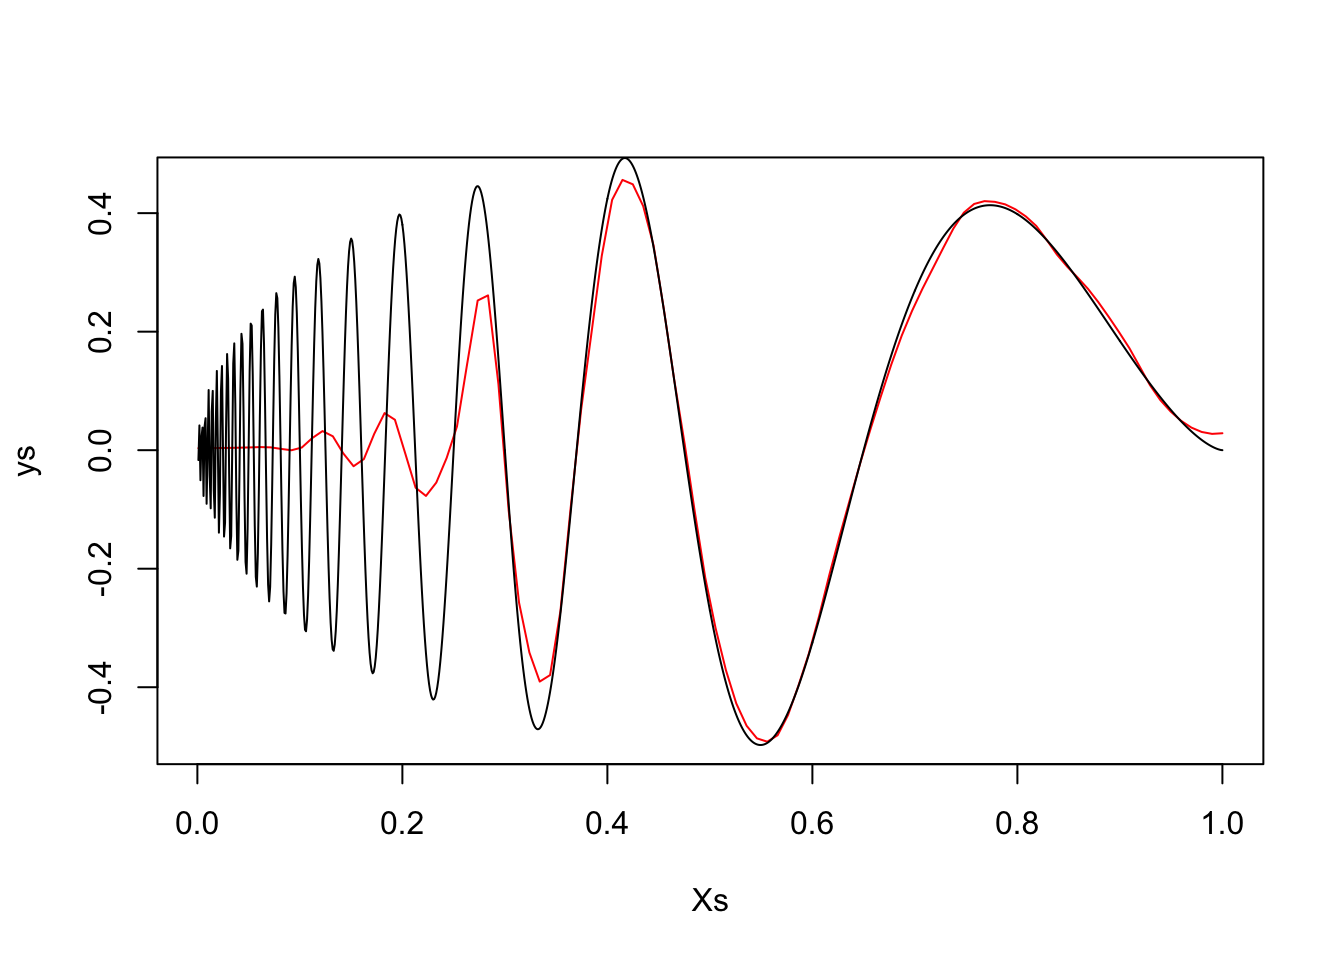
\includegraphics{hw3_files/figure-latex/unnamed-chunk-6-1.pdf}

\begin{Shaded}
\begin{Highlighting}[]
\NormalTok{bstar =}\StringTok{ }\NormalTok{A}\OperatorTok{/}\NormalTok{(A}\OperatorTok{+}\NormalTok{n)}

\NormalTok{## get bhat from simulation}

\NormalTok{risk <-}\StringTok{ }\ControlFlowTok{function}\NormalTok{(b,z,theta)\{}
  \KeywordTok{return}\NormalTok{(}\KeywordTok{sum}\NormalTok{((theta}\OperatorTok{-}\NormalTok{b}\OperatorTok{*}\NormalTok{z)}\OperatorTok{^}\DecValTok{2}\NormalTok{))}
\NormalTok{\}}

\NormalTok{js_exper <-}\StringTok{ }\ControlFlowTok{function}\NormalTok{(seed, theta)\{}
  \KeywordTok{set.seed}\NormalTok{(seed)}
\NormalTok{  n =}\StringTok{ }\KeywordTok{length}\NormalTok{(theta)}
\NormalTok{  z =}\StringTok{ }\KeywordTok{rnorm}\NormalTok{(n,}\DataTypeTok{mean =}\NormalTok{ theta,}\DataTypeTok{sd =} \KeywordTok{replicate}\NormalTok{(n,}\DecValTok{1}\NormalTok{))}
\NormalTok{  bhat =}\StringTok{ }\KeywordTok{max}\NormalTok{(}\DecValTok{0}\NormalTok{,}\DecValTok{1}\OperatorTok{-}\StringTok{ }\NormalTok{(n}\OperatorTok{/}\KeywordTok{sum}\NormalTok{(z}\OperatorTok{^}\DecValTok{2}\NormalTok{)))}
  \KeywordTok{return}\NormalTok{(bhat)}
\NormalTok{\}}

\NormalTok{exper =}\StringTok{ }\DecValTok{1}\OperatorTok{:}\DecValTok{1000}
\NormalTok{Bhat =}\StringTok{ }\KeywordTok{sapply}\NormalTok{(exper, }\ControlFlowTok{function}\NormalTok{(seed) }\KeywordTok{js_exper}\NormalTok{(seed, theta))}
\KeywordTok{plot}\NormalTok{(exper, Bhat, }\DataTypeTok{main =} \StringTok{"simulated bhat vs bstar"}\NormalTok{)}
\KeywordTok{abline}\NormalTok{(}\DataTypeTok{h =}\NormalTok{ bstar, }\DataTypeTok{col =} \StringTok{"red"}\NormalTok{)}
\end{Highlighting}
\end{Shaded}

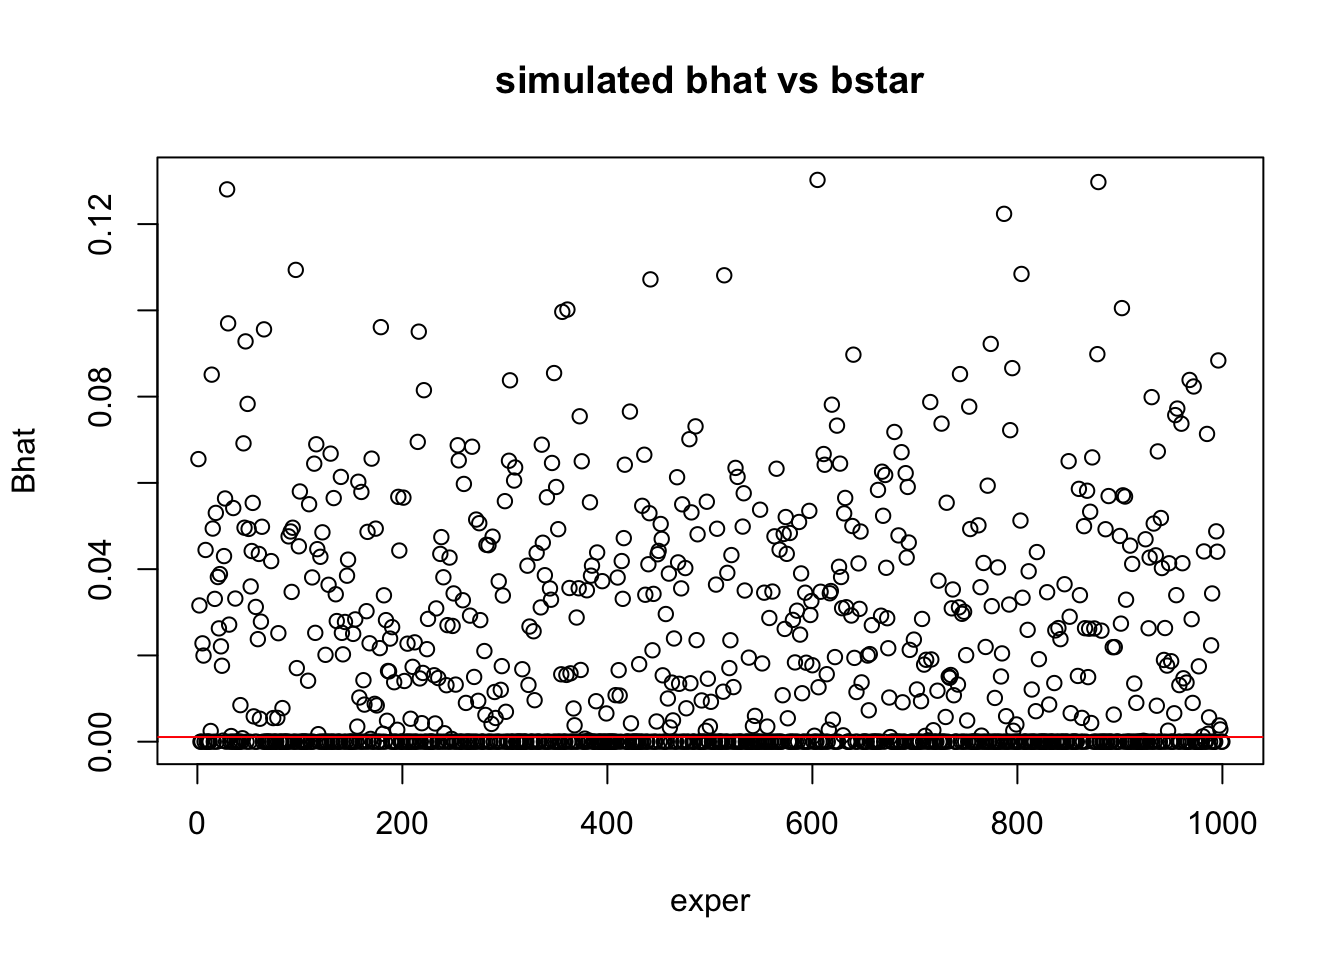
\includegraphics{hw3_files/figure-latex/unnamed-chunk-6-2.pdf}

\begin{Shaded}
\begin{Highlighting}[]
\NormalTok{## compute risk}
\NormalTok{c =}\StringTok{ }\KeywordTok{sum}\NormalTok{(theta}\OperatorTok{^}\DecValTok{2}\NormalTok{)}
\NormalTok{r_B =}\StringTok{ }\KeywordTok{sapply}\NormalTok{(Bhat, }\ControlFlowTok{function}\NormalTok{(bhat) }\KeywordTok{sum}\NormalTok{((theta}\OperatorTok{-}\NormalTok{bhat}\OperatorTok{*}\NormalTok{z)}\OperatorTok{^}\DecValTok{2}\NormalTok{))}
\KeywordTok{plot}\NormalTok{(exper, r_B,}\DataTypeTok{main =} \StringTok{"risk of simulated js vs pinsker"}\NormalTok{)}
\KeywordTok{abline}\NormalTok{(}\DataTypeTok{h =}\NormalTok{ c}\OperatorTok{^}\DecValTok{2}\OperatorTok{/}\NormalTok{(}\DecValTok{1}\OperatorTok{+}\NormalTok{c}\OperatorTok{^}\DecValTok{2}\NormalTok{), }\DataTypeTok{col =} \StringTok{"red"}\NormalTok{)}
\end{Highlighting}
\end{Shaded}

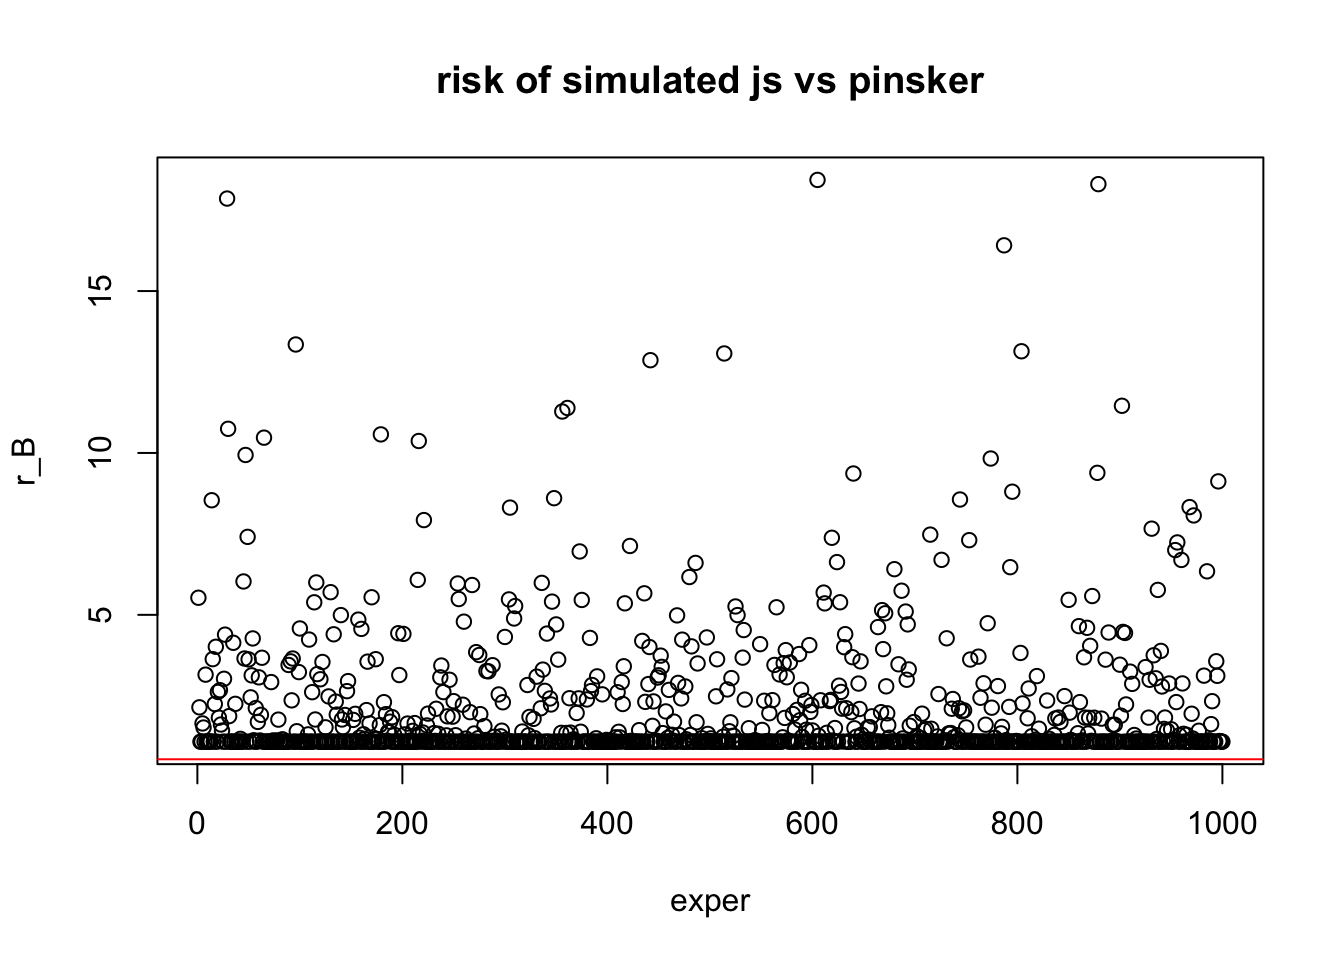
\includegraphics{hw3_files/figure-latex/unnamed-chunk-6-3.pdf}

\begin{Shaded}
\begin{Highlighting}[]
\NormalTok{## finally, use the mean of the simulated bhat as bhat for comparison with MLE  }
\NormalTok{bhat =}\StringTok{ }\KeywordTok{mean}\NormalTok{(Bhat)}

\KeywordTok{print}\NormalTok{(}\KeywordTok{paste0}\NormalTok{(}\StringTok{"mle risk is: "}\NormalTok{, }\KeywordTok{sum}\NormalTok{((theta}\OperatorTok{-}\NormalTok{mle)}\OperatorTok{^}\DecValTok{2}\NormalTok{)))}
\end{Highlighting}
\end{Shaded}

\begin{verbatim}
## [1] "mle risk is: 998.633588966815"
\end{verbatim}

\begin{Shaded}
\begin{Highlighting}[]
\KeywordTok{print}\NormalTok{(}\KeywordTok{paste0}\NormalTok{(}\StringTok{"js risk is: "}\NormalTok{, }\KeywordTok{sum}\NormalTok{((theta}\OperatorTok{-}\NormalTok{bhat}\OperatorTok{*}\NormalTok{z)}\OperatorTok{^}\DecValTok{2}\NormalTok{)))}
\end{Highlighting}
\end{Shaded}

\begin{verbatim}
## [1] "js risk is: 1.33660289209687"
\end{verbatim}

\begin{Shaded}
\begin{Highlighting}[]
\KeywordTok{print}\NormalTok{(}\KeywordTok{paste0}\NormalTok{(}\StringTok{"pinsker bound when c= "}\NormalTok{,c,}\StringTok{" is "}\NormalTok{, c}\OperatorTok{^}\DecValTok{2}\OperatorTok{/}\NormalTok{(}\DecValTok{1}\OperatorTok{+}\NormalTok{c}\OperatorTok{^}\DecValTok{2}\NormalTok{) ))}
\end{Highlighting}
\end{Shaded}

\begin{verbatim}
## [1] "pinsker bound when c= 1.0823232333783 is 0.539472625923871"
\end{verbatim}

\subsection{Comment:}\label{comment-1}

\begin{itemize}
\tightlist
\item
  James-Stein gets better results than MLE.This is because variance is
  much larger than the means, where shrinkage gets advantage over MLE.\\
\item
  James-Stein is bounded by Pinsker bound, which must be true.
\end{itemize}

\section{5}\label{section-1}

\begin{Shaded}
\begin{Highlighting}[]
\NormalTok{data_p5 =}\StringTok{ }\KeywordTok{read.csv}\NormalTok{(}\StringTok{"../data/hw3/assn3-prob5-data.txt"}\NormalTok{, }\DataTypeTok{header =} \OtherTok{FALSE}\NormalTok{)}
\NormalTok{x =}\StringTok{ }\NormalTok{data_p5}\OperatorTok{$}\NormalTok{V1}
\KeywordTok{plot}\NormalTok{(}\KeywordTok{density}\NormalTok{(x))}
\end{Highlighting}
\end{Shaded}

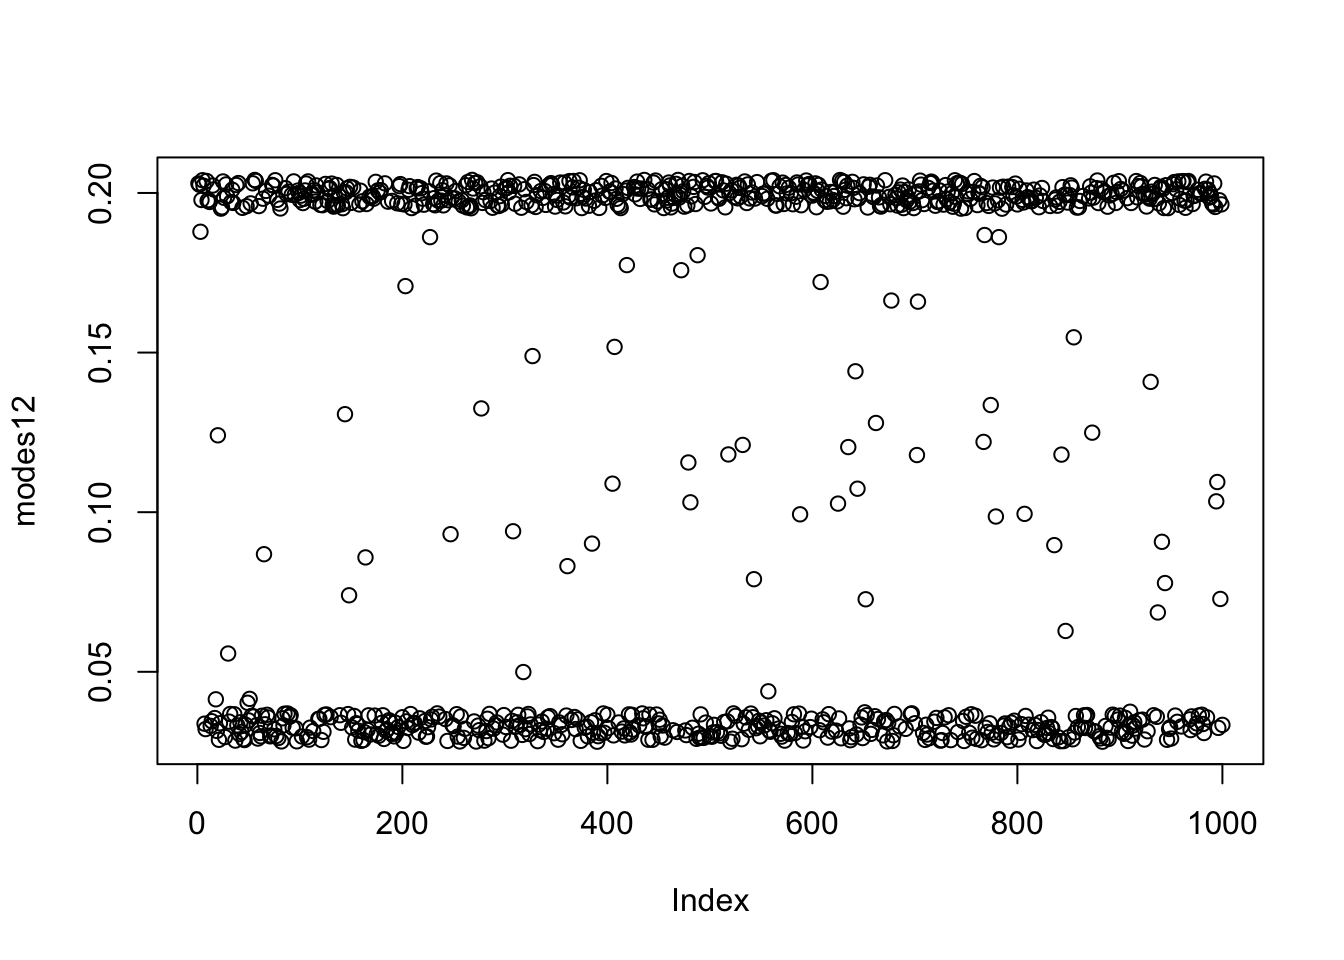
\includegraphics{hw3_files/figure-latex/unnamed-chunk-7-1.pdf}

\begin{Shaded}
\begin{Highlighting}[]
\CommentTok{#lines(density(rpois(100,mean(x))), col = "red")}
\end{Highlighting}
\end{Shaded}

\subsection{estimate sigma}\label{estimate-sigma}

\begin{Shaded}
\begin{Highlighting}[]
\CommentTok{#plot(1:length(x), sort(x, decreasing = TRUE))}
\NormalTok{## take the 25% ~ 75% data and }
\NormalTok{## divide them into smalls bins of length h}
\NormalTok{## get variance for each of the bins and then take the average}

\NormalTok{data_mid =}\StringTok{ }\KeywordTok{sort}\NormalTok{(x, }\DataTypeTok{decreasing =} \OtherTok{TRUE}\NormalTok{)[(}\FloatTok{0.1}\OperatorTok{*}\KeywordTok{length}\NormalTok{(x))}\OperatorTok{:}\NormalTok{(}\FloatTok{0.9}\OperatorTok{*}\KeywordTok{length}\NormalTok{(x))]}
\KeywordTok{plot}\NormalTok{(}\DecValTok{1}\OperatorTok{:}\KeywordTok{length}\NormalTok{(data_mid), data_mid)}
\end{Highlighting}
\end{Shaded}

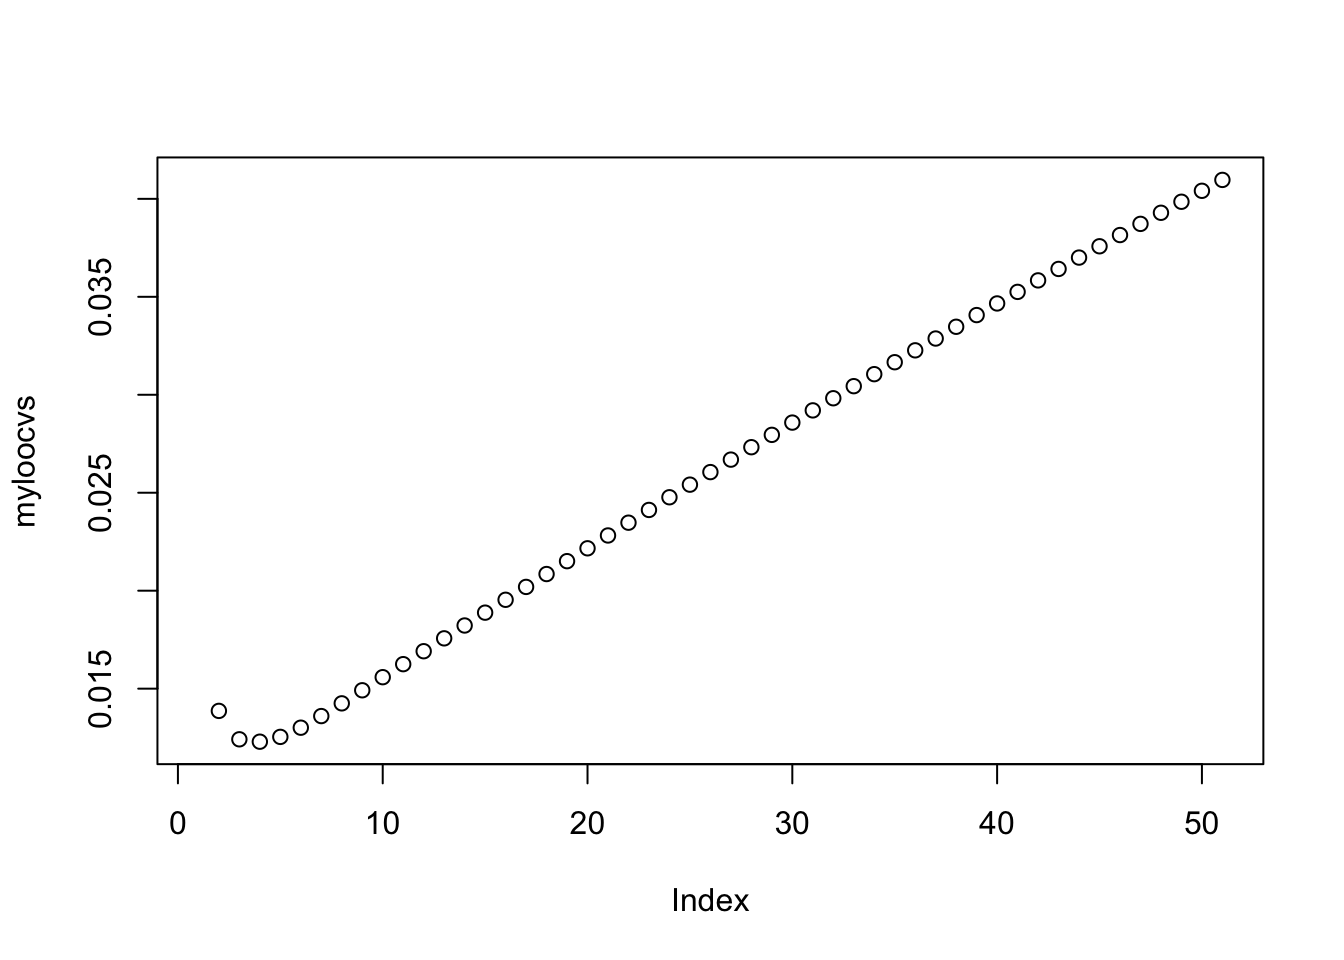
\includegraphics{hw3_files/figure-latex/unnamed-chunk-8-1.pdf}

\begin{Shaded}
\begin{Highlighting}[]
\NormalTok{est_var <-}\StringTok{ }\ControlFlowTok{function}\NormalTok{(}\DataTypeTok{h=}\DecValTok{10}\NormalTok{,}\DataTypeTok{step=}\DecValTok{3}\NormalTok{,}\DataTypeTok{data=}\NormalTok{data_mid)\{}
\NormalTok{  n =}\StringTok{ }\KeywordTok{length}\NormalTok{(data)}
\NormalTok{  Sigma =}\StringTok{ }\KeywordTok{vector}\NormalTok{()}
  \CommentTok{#Diff = vector()}
  \ControlFlowTok{for}\NormalTok{(i }\ControlFlowTok{in} \KeywordTok{seq}\NormalTok{(}\DecValTok{1}\NormalTok{,n}\OperatorTok{-}\NormalTok{h,step))\{}
\NormalTok{    z =}\StringTok{ }\NormalTok{data[i}\OperatorTok{:}\NormalTok{(i}\OperatorTok{+}\NormalTok{h)]}
\NormalTok{    Sigma =}\StringTok{ }\KeywordTok{c}\NormalTok{(Sigma, }\KeywordTok{mean}\NormalTok{((z }\OperatorTok{-}\StringTok{ }\KeywordTok{mean}\NormalTok{(z))}\OperatorTok{^}\DecValTok{2}\NormalTok{))}
    \CommentTok{#Diff = (max(z) -min(z))/mean(z)}
\NormalTok{  \}}
\NormalTok{  sigma =}\StringTok{ }\KeywordTok{mean}\NormalTok{(Sigma)}
  \CommentTok{#diff = mean(Diff)}
  \KeywordTok{return}\NormalTok{(sigma)}
\NormalTok{\}}
\end{Highlighting}
\end{Shaded}

\begin{Shaded}
\begin{Highlighting}[]
\NormalTok{sigma =}\StringTok{ }\KeywordTok{est_var}\NormalTok{(}\DecValTok{50}\NormalTok{)}
\NormalTok{n =}\StringTok{ }\KeywordTok{length}\NormalTok{(x)}
\NormalTok{theta_hat =}\StringTok{ }\KeywordTok{max}\NormalTok{(}\DecValTok{0}\NormalTok{, }\DecValTok{1}\OperatorTok{-}\NormalTok{n}\OperatorTok{*}\NormalTok{sigma}\OperatorTok{^}\DecValTok{2}\OperatorTok{/}\KeywordTok{sum}\NormalTok{(x}\OperatorTok{^}\DecValTok{2}\NormalTok{)) }\OperatorTok{*}\StringTok{ }\NormalTok{x}
\KeywordTok{plot}\NormalTok{(}\KeywordTok{density}\NormalTok{(theta_hat), }\DataTypeTok{main =} \KeywordTok{paste0}\NormalTok{(}\StringTok{"sigma "}\NormalTok{, }\KeywordTok{format}\NormalTok{(sigma,}\DecValTok{4}\NormalTok{), }\StringTok{" b "}\NormalTok{, }\KeywordTok{max}\NormalTok{(}\DecValTok{0}\NormalTok{, }\DecValTok{1}\OperatorTok{-}\NormalTok{n}\OperatorTok{*}\NormalTok{sigma}\OperatorTok{^}\DecValTok{2}\OperatorTok{/}\KeywordTok{sum}\NormalTok{(x}\OperatorTok{^}\DecValTok{2}\NormalTok{))))}
\end{Highlighting}
\end{Shaded}

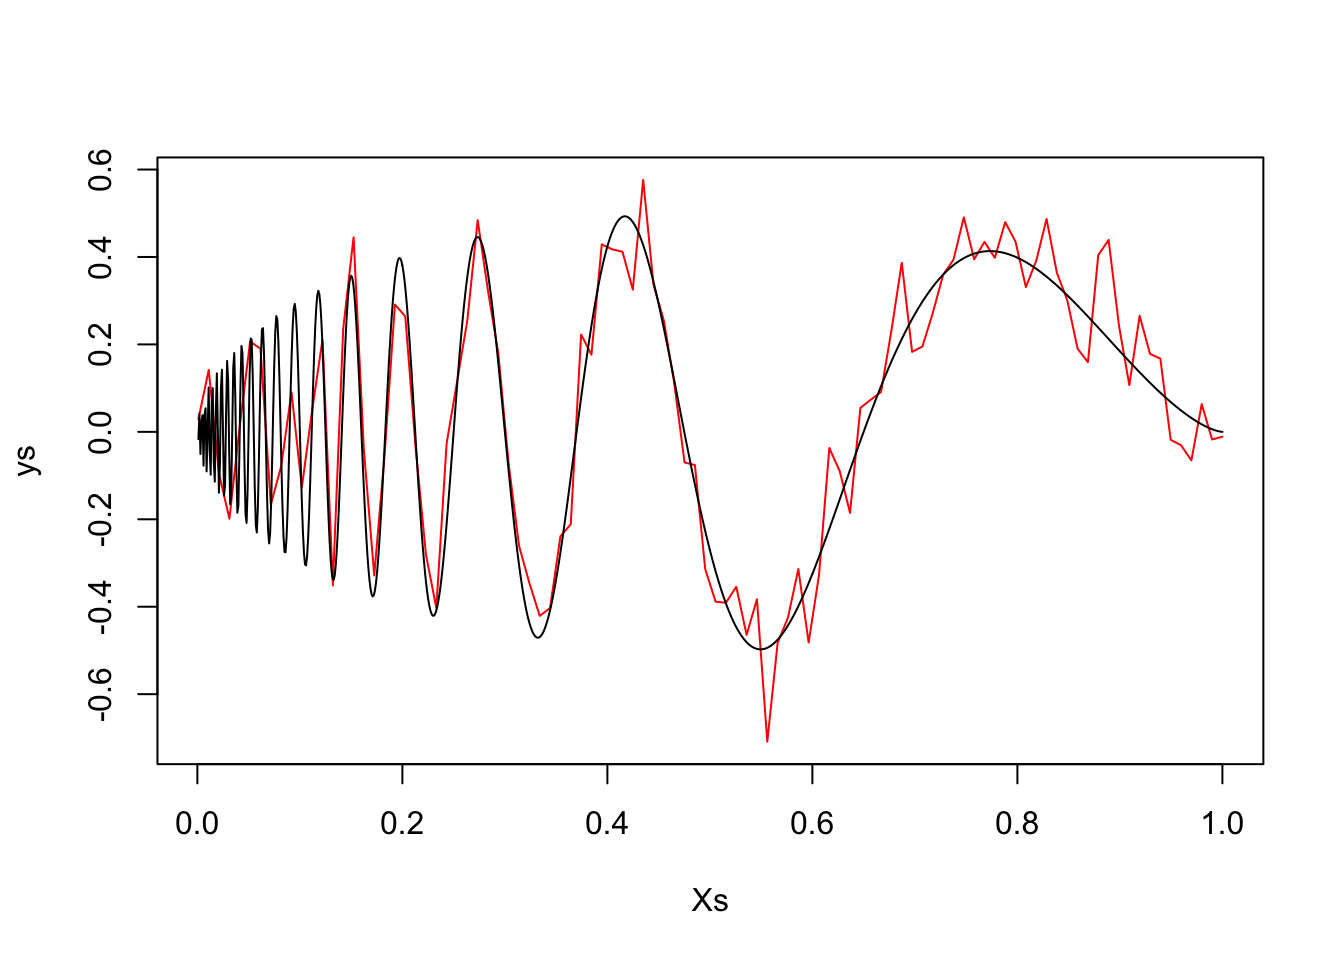
\includegraphics{hw3_files/figure-latex/unnamed-chunk-9-1.pdf}

\begin{Shaded}
\begin{Highlighting}[]
\KeywordTok{write.table}\NormalTok{(theta_hat, }\StringTok{"../data/assn3-wangzh.txt"}\NormalTok{, }\DataTypeTok{row.names =} \OtherTok{FALSE}\NormalTok{, }\DataTypeTok{col.names=}\OtherTok{FALSE}\NormalTok{, }\DataTypeTok{sep =} \StringTok{"}\CharTok{\textbackslash{}n}\StringTok{"}\NormalTok{)}
\end{Highlighting}
\end{Shaded}

\subsection{Comment:}\label{comment-2}

Without any means of validation, this way of estimating variance is like
pure guessing\ldots{}


\end{document}
